\documentclass[11pt]{article}
\usepackage[utf8x]{inputenc}
\usepackage{tikz}
\usetikzlibrary{arrows.meta}
\usetikzlibrary{calc}

%\tikzstyle{age} = [circle, minimum width = 2cm, text centered, draw = black]
%\tikzstyle{arrow} = [thick, ->, >=stealth']

\begin{document}
	\centering
	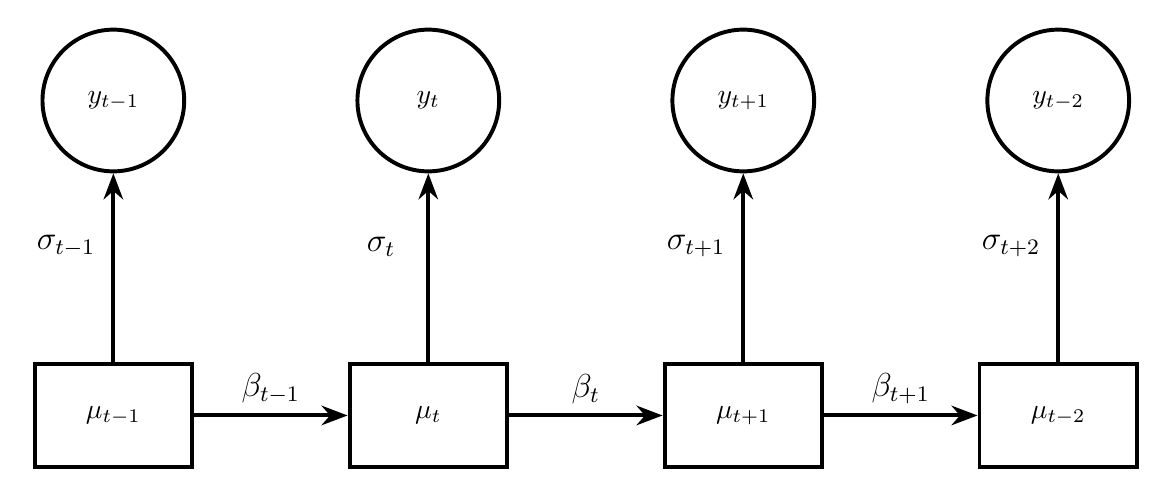
\begin{tikzpicture}[>=Stealth, auto, node distance = 4cm, line width = 0.5mm,
						main node/.style = {rectangle, draw, minimum width = 2cm, minimum height = 1.3cm, line width = 0.5mm},
						obs node/.style = {circle, draw, minimum width = 1.8cm, line width = 0.5mm}]
		\node[main node] (tm1) {$\mu_{t-1}$};
		\node[main node] (t) [right of = tm1] {$\mu_t$};
		\node[main node] (tp1) [right of = t] {$\mu_{t+1}$};
		\node[main node] (tp2) [right of = tp1] {$\mu_{t-2}$};
		
		\node[obs node] (otm1) [above of = tm1]{$y_{t-1}$};
		\node[obs node] (ot) [above of = t] {$y_t$};
		\node[obs node] (otp1) [above of = tp1] {$y_{t+1}$};
		\node[obs node] (otp2) [above of = tp2] {$y_{t-2}$};
		
		\path[->]
		(tm1) edge node [right, anchor = south] {\large $\beta_{t-1}$} (t)
		(t) edge node [right, anchor = south] {\large $\beta_t$} (tp1)
		(tp1) edge node [right, anchor = south] {\large $\beta_{t+1}$} (tp2)
		(tm1) edge node [above, anchor = south, xshift = -0.6cm] {\large $\sigma_{t-1}$} (otm1)
		(t) edge node [above, anchor = south, xshift = -0.6cm] {\large $\sigma_{t}$} (ot)
		(tp1) edge node [above, anchor = south, xshift = -0.6cm] {\large $\sigma_{t+1}$} (otp1)
		(tp2) edge node [above, anchor = south, xshift = -0.6cm] {\large $\sigma_{t+2}$} (otp2);
		%(tp1) edge[loop right] node [anchor = west] {\large $\phi_2$} (ad)
		%\\(ad) edge[bend right] node [left, anchor = south]  {\large $\rho \phi_2$} (fledg)
		%\\(subad) edge[bend left] node [left, anchor = north]  {\large $\rho \phi_2$} (fledg);

	\end{tikzpicture}
\end{document}
